\documentclass[polish,polish,a4paper]{article}
\usepackage[T1]{fontenc}
\usepackage[utf8]{inputenc}
\usepackage{babel}
\usepackage{amsmath}
\usepackage{subcaption}
\usepackage{anysize}
\usepackage{url}
\usepackage{pdfpages}
\usepackage{listings}
\usepackage{ucs}
\usepackage{xcolor}

\marginsize{2.5cm}{2.5cm}{1.75cm}{1.75cm}

\definecolor{codecomment}{rgb}{0,0.5,0}
\definecolor{codekeyword}{rgb}{0,0,1}
\definecolor{codestring}{rgb}{0.64,0.08,0.08}

\lstdefinestyle{mystyle}{
	commentstyle=\color{codecomment}\textit,
	keywordstyle=\color{codekeyword},
	stringstyle=\color{codestring},
	numberstyle=\color{gray},
	basicstyle=\ttfamily,
	captionpos=b,
	tabsize=4,
	numbers=left,
	numbersep=12pt,
	xleftmargin=36pt,
	breaklines=true,
	escapechar=|
}

\lstset{style=mystyle}

\lstset{
	inputencoding=utf8x, 
	extendedchars=\true,
	literate={ą}{{\k{a}}}1
	{Ą}{{\k{A}}}1
	{ę}{{\k{e}}}1
	{Ę}{{\k{E}}}1
	{ó}{{\'o}}1
	{Ó}{{\'O}}1
	{ś}{{\'s}}1
	{Ś}{{\'S}}1
	{ł}{{\l{}}}1
	{Ł}{{\L{}}}1
	{ż}{{\.z}}1
	{Ż}{{\.Z}}1
	{ź}{{\'z}}1
	{Ź}{{\'Z}}1
	{ć}{{\'c}}1
	{Ć}{{\'C}}1
	{ń}{{\'n}}1
	{Ń}{{\'N}}1
}

\begin{document}
	
	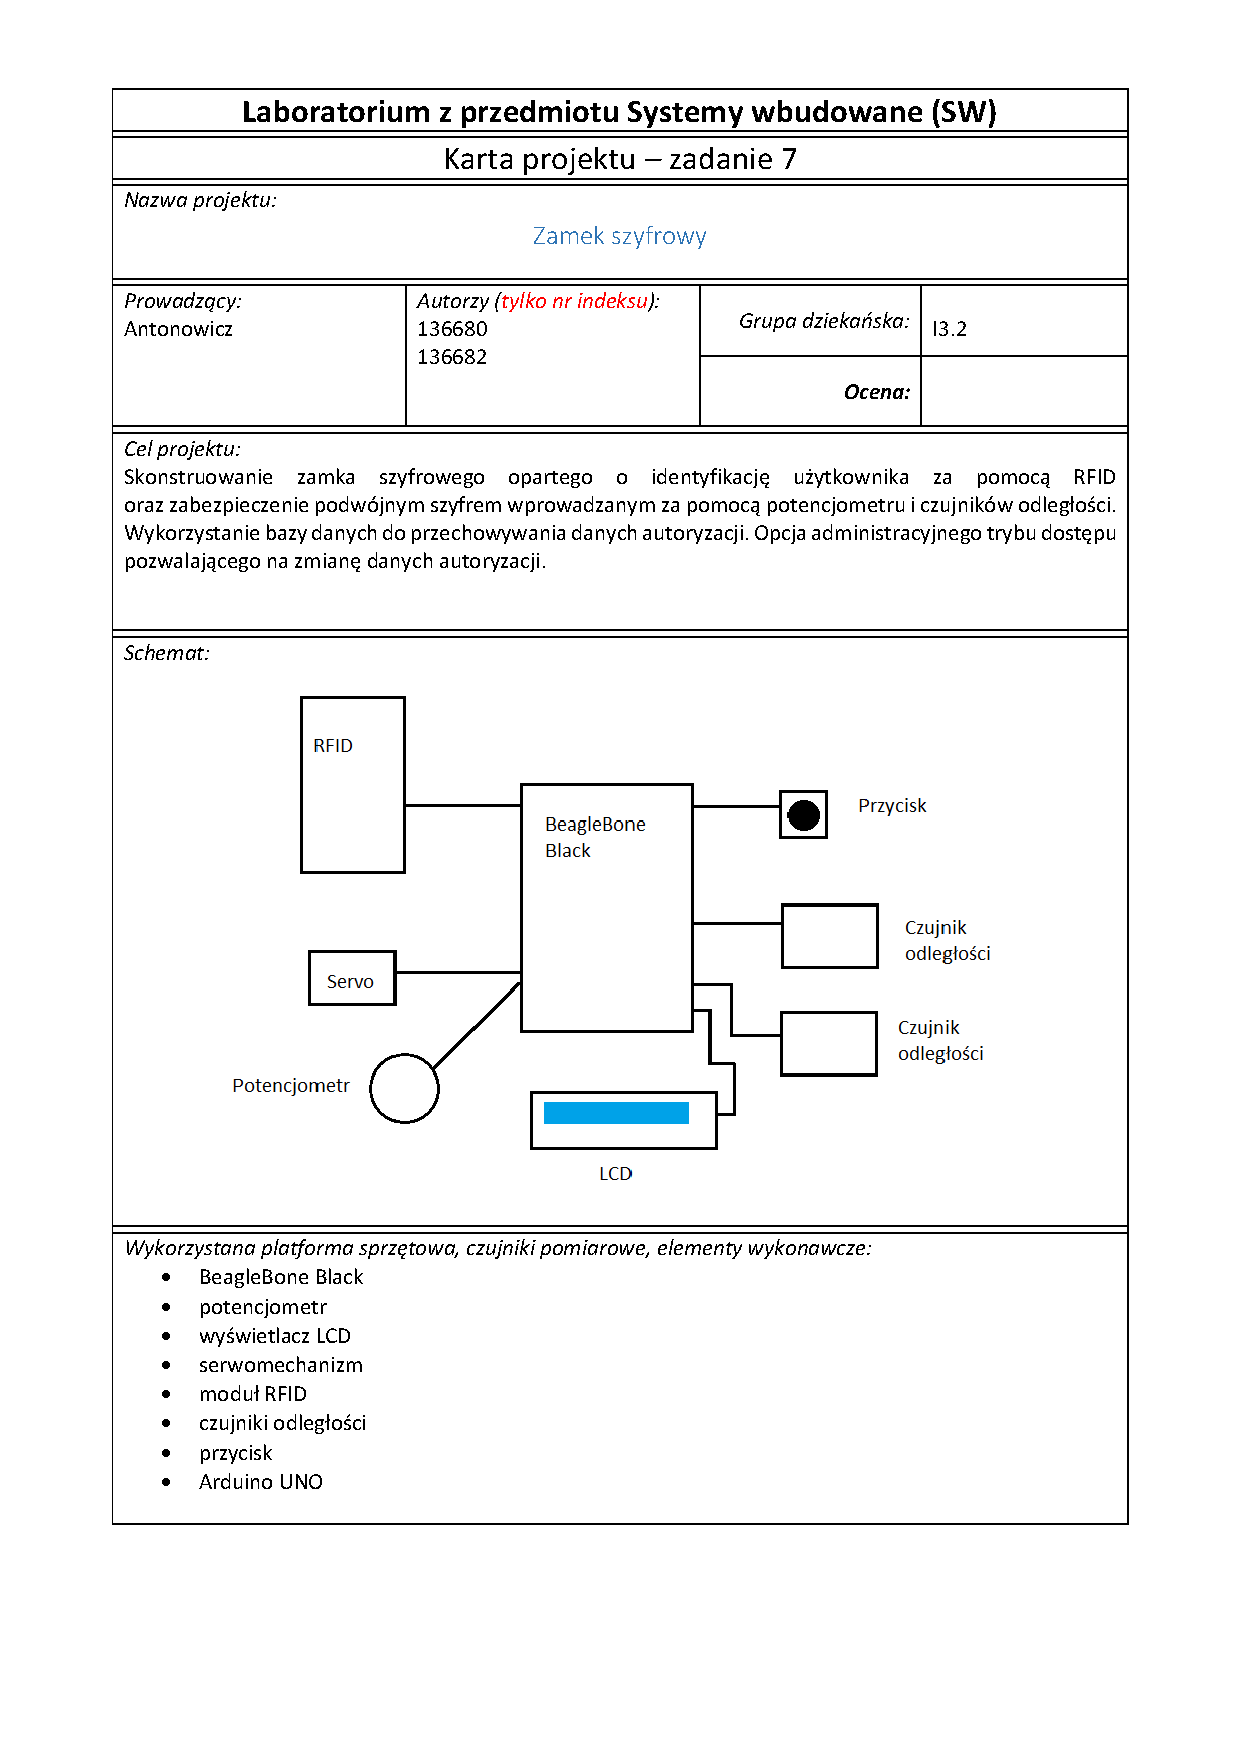
\includepdf{SW_KARTA_PROJ.pdf}
	
	\section{Zakres projektu}
	%TODO
	
	\section{Realizacja}
	%TODO: Schemat i zdjęcie całego układu z krótkim opisem
	
	\subsection{Interakcja z użytkownikiem}
	\label{scenario}
	Interakcja systemu z użytkownikiem przebiega następująco:
	\begin{enumerate}
		\item Użytkownik identyfikuje się za pomocą prywatnego transpondera RFID.
		\item System weryfikuje użytkownika i wyświetla komunikat z żądaniem wprowadzenia szyfru podstawowego.
		\item Użytkownik wprowadza szyfr podstawowy za pomocą układu potencjometru.
		\item System sprawdza poprawność szyfru i wyświetla komunikat z żądaniem wprowadzenia szyfru drugorzędnego.
		\item Użytkownik wprowadza szyfr drugorzędny za pomocą układu czujników odległości.
		\item System sprawdza poprawność szyfru i otwiera zamek.
		\item Użytkownik zamyka zamek przez naciśnięcie przycisku.
	\end{enumerate}
	Możliwy jest również alternatywny scenariusz, w którym odebrany przez czytnik RFID identyfikator należy do administratora systemu:
	\begin{enumerate}
		\item Administrator identyfikuje się za pomocą transpondera RFID.
		\item System weryfikuje użytkownika i przełącza się w tryb administracyjny.
		\item System odczytuje za pomocą czytnika RFID identyfikator użytkownika, dla którego mają zostać wprowadzone nowe kody dostępu.
		\item System wyświetla komunikat z żądaniem utworzenia szyfru podstawowego.
		\item Użytkownik wprowadza nowy szyfr podstawowy za pomocą układu potencjometru.
		\item System wyświetla komunikat z żądaniem potwierdzenia nowego szyfru.
		\item Użytkownik ponownie wprowadza szyfr podstawowy z kroku 5.
		\item System sprawdza poprawność szyfru i wyświetla komunikat z żądaniem utworzenia szyfru drugorzędnego.
		\item Użytkownik wprowadza nowy szyfr drugorzędny za pomocą układu czujników odległości.
		\item System wyświetla komunikat z żądaniem potwierdzenia nowego szyfru.
		\item Użytkownik ponownie wprowadza szyfr podstawowy z kroku 9.
		\item System sprawdza poprawność szyfru i zapisuje nowe dane uwierzytelniania.
		\item System przełącza się w tryb podstawowy.
	\end{enumerate}
	Zmiana kodów dostępu jest również możliwa bez udziału administratora, jeśli zamek jest w danym momencie otwarty, a transponder użytkownika zostanie ponownie odczytany. W tym przypadku procedura zmiany danych uwierzytelniania przebiega zgodnie z punktami 3--12 scenariusza dostępu administracyjnego.
	
	\noindent\\
	Komunikaty systemu prezentowane są użytkownikowi za pomocą układu wyświetlacza LCD podłączonego do platformy Arduino UNO, obsługiwanego przy pomocy biblioteki \verb|LiquidCrystal_I2C.h| wykorzystującej protokół I2C do komunikacji z urządzeniem. Tekst do wyświetlenia jest przesyłany z programu głównego, uruchomionego na platformie BeagleBone Black, za pośrednictwem UART.
	
	\subsection{Identyfikacja użytkownika}
	Identyfikacja polega na odczycie przez czytnik RFID numeru UID transpondera użytkownika. Czytnik jest podłączony do platformy Arduino UNO i obsługiwany poprzez protokół SPI za pośrednictwem bibliotek \verb|SPI.h| oraz \verb|MFRC522.h|. Po wykryciu transpondera następuje odczytanie numeru identyfikacyjnego i przesłanie go do programu głównego za pośrednictwem UART. Następnie wykonane zostaje zapytanie do bazy danych, które pozwala stwierdzić, czy użytkownik o danym UID jest zarejestrowany w systemie, a także czy posiada on status administratora.
	
	\subsection{Uwierzytelnianie}
	Projekt zawiera dwa mechanizmy uwierzytelniania użytkownika, uruchamiane kolejno, bezpośrednio po pomyślnej identyfikacji. Pierwszy z nich polega na wprowadzeniu szyfru za pomocą potencjometru, przekręcając jego gałkę na przemian zgodnie i przeciwnie do ruchu wskazówek zegara. Każda zmiana kierunku obrotu, przy pewnej ustalonej dokładności odczytu, powoduje wprowadzenie pojedynczej cyfry szyfru. Kod definiujący proces wprowadzania szyfru podstawowego został przedstawiony na listingu \ref{pass0}.
	\begin{lstlisting}[language=Python, caption={Fragment kodu sterującego wprowadzaniem szyfru podstawowego}, label=pass0]
def read():
	# Inicjalizacja
	[...]
	passcode = ''
	# Pętla odczytująca kolejne znaki
	while len(passcode) < passcodeLength:
		# Odczyt wartości napięcia z potencjometru
		v = read_value()
		previousState = state
		# Odczytana wartość jest większa od dolnego progu|\linebreak|dla cyfry większej o 1
		if state < nSegments - 1 and v > lb[state+1]:
			if direction < 0:
				passcode += hex(state)[2]
			state += 1
			direction = 1
		# Odczytana wartość jest mniejsza od górnego progu|\linebreak|dla cyfry mniejszej o 1
		elif state > 0 and v < ub[state-1]:
			if direction > 0:
				passcode += hex(state)[2]
			state -= 1
			direction = -1
	return passcode
	\end{lstlisting}
	Szyfr drugorzędny jest wprowadzany za pomocą czujników odległości. Kolejne cyfry są generowane na podstawie numeru czujnika oraz wartości odczytanej przez niego odległości. Kod definiujący proces wprowadzania szyfru drugorzędnego został przedstawiony na listingu \ref{pass1}.
	\begin{lstlisting}[language=Python, caption={Fragment kodu sterującego wprowadzaniem szyfru drugorzędnego}, label=pass1]
def read():
	# Inicjalizacja
	[...]
	passcode = ''
	# Pętla odczytująca kolejne znaki
	while len(passcode) < passcodeLength:
		# Pętla iterująca po stanach kolejnych czujników
		for i, state in enumerate(states):
			# Odczyt odległości z czujnika o numerze i
			v = read_value(i)
			# Kwantyzacja wartości odległości
			newState = states[i] = bisect(bounds, v)
			if state == nSegments and newState < nSegments:
				passcode += hex(i * nSegments + newState)[2]
	return passcode
	\end{lstlisting}
	Obydwa układy są podłączone do platformy BeagleBone Black i obsługiwane za pomocą bibliotek \linebreak\verb|Adafruit_BBIO.ADC| oraz \verb|Adafruit_BBIO.GPIO|.
	
	\subsection{Sterowanie zamkiem}
	W zaprojektowanym układzie funkcję zamka pełni serwomechanizm, który jest przełączany pomiędzy stanami odpowiadającymi otwarciu i zamknięciu zamka. Do jego obsługi wykorzystano bibliotekę \linebreak\verb|Adafruit_BBIO.PWM|. Zgodnie ze scenariuszem opisanym w sekcji \ref{scenario}, zamek otwiera się po pomyślnym uwierzytelnieniu użytkownika, natomiast jego zamknięcie następuje po naciśnięciu przycisku. Stan przycisku jest odczytywany przez program za pomocą biblioteki \verb|Adafruit_BBIO.GPIO|.
	
	\subsection{Sposób przechowywania danych}
	Dane wykorzystywane do uwierzytelniania i autoryzacji użytkowników przechowywane są w bazie danych SQLite. Na jej schemat składają się trzy relacje:
	\begin{itemize}
		\item \verb|users|, zawierająca rekordy opisujące użytkowników (identyfikator, wartości funkcji haszujących dla kodów dostępu, przypisany numer zamka),
		\item \verb|admins|, zawierająca rekordy z identyfikatorami administratorów systemu,
		\item \verb|logs|, zawierająca rekordy opisujące próby dostępu do systemu (czas dostępu, identyfikator użytkownika, status).
	\end{itemize}
	%TODO: Schemat bazy danych
	
	\section{Wnioski}
	%TODO
	
\end{document}
